\themaM
\graphicspath{{../../S19_Volume_du_prisme_et_du_cylindre/Images/}}

\chapter{Volume du prisme\\et du cylindre}
\label{S19}


%%%%%%%%%%%%%%%%%%%%%%%%%%%%%%
%%%%%%%%%%%%%%%%%%%%%%%%%%%%%%
\begin{autoeval}
   \small
   \begin{enumerate}
      \item Il calcule le volume d'un pavé droit, d'un prisme droit, d'un cylindre.
      \item Il calcule le volume d'un assemblage de ces solides.
      \item Il effectue des conversions d’unités de volumes.
      \item Il utilise la correspondance entre les unités de volume et de contenance (\ul{1} = \udmc{1} , \ul{1000} = \umc{1}) pour effectuer des conversions.
   \end{enumerate}
\end{autoeval}

\begin{prerequis}
   \begin{itemize}
      \item Volume d'un prisme, d'un cylindre.
      \item Correspondance entre volume et contenance : \\
         $\ul{1} =\udmc{1}$ et $\ul{1000} =\umc{1}$.
      \item[\com] Vérifier le cohérence des résultats au niveau des unités.
      \item[\com] Effectuer des conversions d'unités de volumes.
   \end{itemize}
\end{prerequis}

\vfill

\begin{debat}[Débat : $\ul{1} =\udmc{1}$]
   Cette correspondance est à connaître. Pourtant, elle ne paraît pas si naturelle que cela : elle signifie que l'eau contenue dans une bouteille d'un litre remplirait exactement un cube de \udm{1} de côté.
   \begin{center}
      {\psset{unit=0.9}
      \begin{pspicture}(0,0)(6,5.5)
         \psline(0.5,0.5)(0.5,3.75) %bouteille
         \psline(2,0.5)(2,3.75)
         \psarc(1.5,3.75){0.5}{0}{90}
         \psarc(1,3.75){0.5}{90}{180}
         \psline(1,4.25)(1,5)
         \psline(1.5,4.25)(1.5,5)
         \psellipticarc(1.25,0.5)(0.75,0.3){180}{0}
         \psellipticarc(1.25,3.5)(0.75,0.3){180}{0}
         \psellipticarc[linestyle=dashed](1.25,3.5)(0.75,0.3){0}{180}
         \psellipse(1.25,5)(0.25,0.1)
         \rput(1.25,2){\textcolor{B1}{\ul{1}}}
         \psframe(3,0.5)(5,2.5) %cube
         \psline(3,2.5)(3.75,3.25)(5.75,3.25)(5.75,1.25)(5,0.5)
         \psline(5,2.5)(5.75,3.25)
         \rput(4,0.2){\textcolor{B1}{$\udm{1} =\ucm{10}$}}
         \rput(4,1.5){\textcolor{B1}{$\udmc{1}$}}
      \end{pspicture}}
   \end{center}
   \bigskip
   \begin{cadre}[B2][J4]
      \begin{center}
         Vidéo : \href{https://www.yout-ube.com/watch?v=DRKmlWtUN0k}{\bf Correspondance entre unités de volume et de contenance}, chaîne de {\it Jean-Charles Toussaint}.
      \end{center}
   \end{cadre}
\end{debat}


%%%%%%%%%%%%%%%%%%%%%%%%%%%%%%
%%%%%%%%%%%%%%%%%%%%%%%%%%%%%%
\activites

\begin{activite}[Des pavés cachés]
   {\bf Objectifs :} calculer le volume d'un pavé droit, d'un assemblage de solides ; résoudre un problème dans le domaine des grandeurs et mesures. \\
      {\bf Matériel à disposition :} des cubes à emboiter, des briques types kapla ou Lego, des boites, des morceaux de sucres.
   \begin{QCM}
      \partie[On me voit assez bien !]
         \begin{minipage}{11.5cm}
            Ma petite sœur empile des cubes les uns sur les autres, tous de même forme. Voici sa construction. \\
            Combien a-t-elle empilé de cubes ? \\ [1.5cm]
         \end{minipage}
         \qquad
         \begin{minipage}{4.5cm}
            \includegraphics[width=4cm]{assemblage_cubes}
         \end{minipage}
         
      \partie[On me voit un peu moins !]
         \begin{minipage}{9cm}
            Mon grand-père veut construire la même jardinière que sur la photo ci-contre. \\
            De combien de briques aura-t-il besoin ? \\ [2cm]
         \end{minipage}
         \qquad
         \begin{minipage}{7cm}
            \includegraphics[width=6.5cm]{jardiniere}
         \end{minipage}
         
      \partie[On ne me voit plus !]
         L’entreprise Sucromania fabrique du sucre en morceaux. Elle souhaite conditionner ses morceaux dans un emballage parallélépipédique de \umm{280} de long, \umm{140} de large et \umm{70} de hauteur. \\
         Sachant qu’un sucre a la forme d’un pavé droit de \umm{14} de long, \umm{14} de large et \umm{10} de hauteur, combien de sucres peut-elle mettre au maximum afin d’optimiser son emballage ? \\ [5cm] 
   \end{QCM}
   
   \vfill \hfill {\it\footnotesize Source : d'après \href{https://eduscol.education.fr/document/13132/download}{\og La résolution de problèmes mathématiques au collège}, MENJS, p.136}
\end{activite}


%%%%%%%%%%%%%%%%%%%%%%%%%%%%%%
%%%%%%%%%%%%%%%%%%%%%%%%%%%%%%
\cours 

%%%%%%%%%%%%%%%%%%
\section{Volume par dénombrement}

\begin{definition}
   Le \textbf{volume} est une grandeur physique qui mesure l'espace occupé par celui-ci.
\end{definition}

\begin{exemple*1}
   {\psset{unit=0.5}
   Ces trois objets n'ont pas la même forme mais occupent la même quantité d'espace, ils ont donc le même volume.
   \begin{center}
      \begin{pspicture}(0,-1)(13,3.5)
         \psset{linecolor=A1}
         \psframe(0,0)(3,2)
         \psline(1,0)(1,2)(1.5,2.5)
         \psline(2,0)(2,2)(2.5,2.5)
         \psline(0,1)(3,1)(3.5,1.5)
         \psline(3,0)(3.5,0.5)(3.5,2.5)(0.5,2.5)(0,2)
         \psline(3,2)(3.5,2.5)
         \psset{linecolor=B1}
         \pspolygon(5,0)(9,0)(9,2)(8,2)(8,1)(6,1)(6,2)(5,2)
         \psline(5,1)(6,1)(6,0)
         \psline(7,0)(7,1)(7.5,1.5)
         \psline(9,0)(9.5,0.5)(9.5,2.5)(8.5,2.5)(8,2)
         \psline(9,2)(9.5,2.5)
         \psline(9.5,1.5)(9,1)(8,1)(8,0)
         \psline(5,2)(5.5,2.5)(6.5,2.5)(6.5,1.5)(8,1.5)
         \psline(6,2)(6.5,2.5)
         \psline(6,1)(6.5,1.5)    
         \psset{linecolor=G1}  
         \pspolygon(11,0)(14,0)(14,1)(13,1)(13,2)(12,2)(12,3)(11,3)
         \psline(12,0)(12,1)(11,1)
         \psline(13,0)(13,1)(12,1)(12,2)(11,2)
         \psline(14,0)(14.5,0.5)(14.5,1.5)(13.5,1.5)(13.5,2.5)(12.5,2.5)(12.5,3.5)(11.5,3.5)(11,3)
         \psline(14,1)(14.5,1.5)
         \psline(13,2)(13.5,2.5)
         \psline(12,3)(12.5,3.5)
         \psline(13,1)(13.5,1.5)
         \psline(12,2)(12.5,2.5)
      \end{pspicture}
   \end{center}
   Si l'unité de volume est un cube \psline(0,1)(0,0)(1,0)(1,1)(0,1)(0.5,1.5)(1.5,1.5)(1.5,0.5)(1,0) \psline(1,1)(1.5,1.5) \hfill le volume de ces trois solides est de 6 unités de volume.}
\end{exemple*1}

\bigskip

Il existe deux unités en dimension 3 : les unités de volumes en \og cube \fg{} et les unités de capacité en \og litre \fg. 

\begin{definition}
   \begin{itemize}
      \item Lorsque l'unité de volume est un cube de \um{1} d'arête, cela représente \umc{1}.
      \item Le {\bf litre} (L) est une unité de capacité valant \udmc{1}. On a alors $\ul{1} =\udmc{1}$ et $\ul{1000} =\umc{1}$.
   \end{itemize}
   \vspace*{-4mm}
\end{definition}

\bigskip

Pour effectuer un changement d'unité de volume, on reprend les même préfixes que pour les changements de longueur, et on impose pour chacun d'eux trois colonnes au tableau. \smallskip

\Tableau[Cube,Capacite,FlechesH]{39621/12}
\vspace*{-8mm}

\begin{exemple*1}
    \udamc{0,0039621} = \umc{3,9621} = \udmc{3962,1} = \ul{3962,1} = \ucmc{3962100}.
\end{exemple*1}
   
   
%%%%%%%%%%%%%%%
\section{Volumes classiques}

\begin{minipage}[t]{5.5cm}
   \Formule[Volume,Solide=pave,Largeur=5.5cm,Ancre={(2.75,-2)},Couleur=yellow!10]
\end{minipage}
\qquad
\begin{minipage}[t]{4.5cm}
   \Formule[Volume,Solide=prisme,Largeur=4.5cm,Ancre={(2.25,-2)},Couleur=yellow!10]
\end{minipage}
\qquad
\begin{minipage}[t]{6cm}
   \Formule[Volume,Solide=cylindre,Largeur=6cm,Ancre={(3,-2)},Couleur=yellow!10]
\end{minipage}


%%%%%%%%%%%%%%%%%%%% %%%%%%%%%
%%%%%%%%%%%%%%%%%%%% %%%%%%%%%
\exercicesbase

\begin{colonne*exercice}

\begin{exercice} %1
   Donner le volume de chaque solide en unités de volume (les volumes sont supposés pleins).
   \begin{center}
      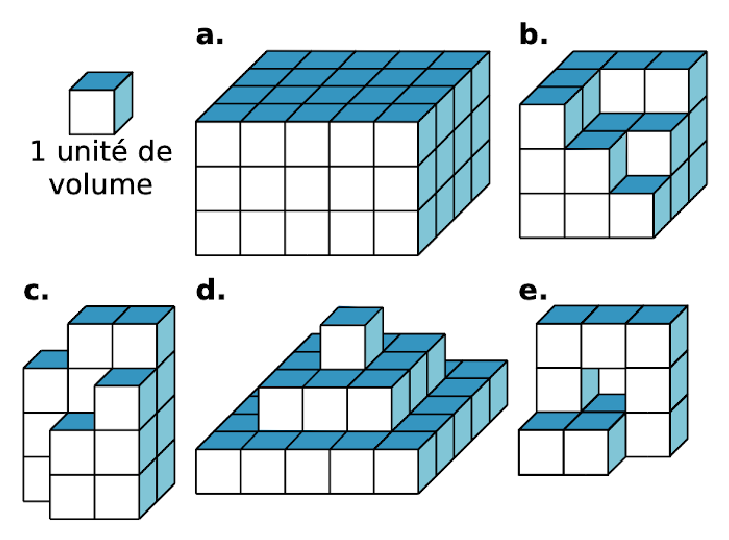
\includegraphics[width=7cm]{cubes}
   \end{center}
\end{exercice}

\begin{corrige}
  On note u l'unité de volume. \\
  \begin{enumerate}
     \item $5\times4\times3 =60$. Donc, {\blue a = 60 u}.
     \item $3^{3}-(4+1) =27-5 =22$. Donc, {\blue b = 22 u}.
     \item $7+6+3 =16$. Donc, {\blue c = 16 u}.
     \item $5^{3}+3^{3}+1 =25+9+1 =$. Donc, {\blue d = 35 u}.
     \item $8+2 =10$. Donc, {\blue e = 10 u}.
  \end{enumerate}
\end{corrige}

\smallskip


\begin{exercice} %2
   Classer ces pavés du plus petit au plus grand volume.
   \begin{center}
      {\psset{unit=0.5,fillstyle=solid,fillcolor=lightgray}
      \footnotesize
      \begin{pspicture}(1,0.5)(11,8)
         \pspolygon(1,1)(5,1)(6,2)(6,3.5)(2,3.55)(1,2.5)
         \psline(1,2.5)(5,2.5)(6,3.5)
         \psline(5,2.5)(5,1)
         \rput(3,0.6){\ucm{4}}
         \rput{90}(0.6,1.75){\ucm{1,5}}
         \rput{45}(5.8,1.2){\ucm{2,5}}
         \rput(3.5,3){C}
         \pspolygon(1,5)(3.5,5)(4.5,6)(4.5,8.5)(2,8.5)(1,7.5)
         \psline(1,7.5)(3.5,7.5)(4.5,8.5)
         \psline(3.5,7.5)(3.5,5)
         \rput(2.25,4.6){\ucm{2,5}}
         \rput(2.25,6.25){cube}
         \rput(2.5,8){A}
         \pspolygon(9,1)(10,1)(10.9,1.9)(10.9,8.9)(9.9,8.9)(9,8)
         \psline(10,1)(10,8)(10.9,8.9)
         \psline(10,8)(9,8)
         \rput(9.4,0.6){\ucm{1}}
         \rput{45}(10.9,1.15){\ucm{2,2}}
         \rput{90}(8.6,4.5){\ucm{7}}
         \rput(10,8.5){B}
      \end{pspicture}}
   \end{center}
\end{exercice}

\begin{corrige}
\ \\ [-5mm]
   \begin{itemize}
      \item Le volume du cube A vaut $c^3$ : \\
      $V_{\text A} =\ucm{2,5}\times\ucm{2,5}\times\ucm{2,5} ={\blue \ucmc{15,625}}$.
      \item Le volume du pavé haut B vaut $L\times\ell\times h$ : \\
      $V_{\text B} =\ucm{2,2}\times\ucm{1}\times\ucm{7} ={\blue \ucmc{15,4}}$.
      \item Le volume du dernier pavé C vaut $L\times\ell\times h$ : \\
      $V_{\text C} =\ucm{4}\times\ucm{2,5}\times\ucm{1,5} ={\blue \ucmc{15}}$.
   \end{itemize}
   On a donc {\blue C < B < A}. \\
\end{corrige}

\smallskip


\begin{exercice} %3
   Associer à chaque mesure l'objet qui lui correspond.   
   \Relie[LargeurG=19mm,Ecart=7mm,LargeurD=32mm,Stretch=1.1]
      {\ul{16}/Maison/2,
      \uhmc{1}/Cartable/6,
      \ummc{10}/Baignoire/7,
      \umc{600}/Mer Méditerranée/6,
      \ukmc{3700000}/Bille/4,
      \ucmc{1}/Empire State Building/5,
      \ul{160}/Grain de riz/3}
\end{exercice}

\begin{corrige}
\ \\ [-4mm]
   \Relie[Solution,Couleur=blue,LargeurG=18mm,Ecart=8mm,LargeurD=32mm,Stretch=1.1]
      {\ul{16}/Maison/2,
      \uhmc{1}/Cartable/6,
      \ummc{10}/Baignoire/7,
      \umc{600}/Mer Méditerranée/1,
      \ukmc{3700000}/Bille/4,
      \ucmc{1}/Empire State Building/5,
      \ul{160}/Grain de riz/3}
\end{corrige}
   
\smallskip


\begin{exercice} %4
   Effectuer les conversions de volumes et capacités : \smallskip
   \begin{enumerate}
      \item \udmc{1} = \pointilles \ummc{} \smallskip
      \item \ummc{200} = \pointilles \ucmc{} \smallskip
      \item \ukmc{1542} = \pointilles \udamc{} \smallskip
      \item \ul{1} = \pointilles \udl{} \smallskip
      \item \udal{1,53} = \pointilles \ucl{} \smallskip
      \item \udl{35} = \pointilles \ul{} \smallskip
      \item \uhl{1} = \pointilles \ucmc{} \smallskip
      \item \ul{131,2} = \pointilles \umc{} \smallskip
      \item \ucmc{35,635} = \pointilles \udl{} \smallskip
   \end{enumerate}
\end{exercice}

\begin{corrige}
\ \\ [-5mm]
   \begin{enumerate}
      \item \udmc{1} = \textcolor{blue}{1\,000\,000} \ummc{}
      \item \ummc{200} = \textcolor{blue}{0,2} \ucmc{}
      \item \ukmc{1542} = \textcolor{blue}{1\,542\,000\,000} \udamc{}
      \item \ul{1} = \textcolor{blue}{10} \udl{}
      \item \udal{1,53} = \textcolor{blue}{1\,530} \ucl{}
      \item \udl{35} = \textcolor{blue}{3,5} \ul{}
      \item \uhl{1} = \textcolor{blue}{100\,000} \ucmc{}
      \item \ul{131,2} = \textcolor{blue}{0,1\,312} \umc{}
      \item \ucmc{35,635} = \textcolor{blue}{0,35\,635} \udl{}
   \end{enumerate}
\end{corrige}

\smallskip


\begin{exercice} %5
   Dans chacune des figures suivantes, colorier une base en jaune, repasser une hauteur en rouge puis calculer le volume.
   \begin{center}
      \includegraphics[width=65mm]{prismes_cylindres}
   \end{center}
\end{exercice}

\begin{corrige}
   \begin{itemize}
      \item $V_a =\ucmq{8}\times\ucm{6,5} ={\blue \ucmc{52}}$ \smallskip
      \item $V_b =\dfrac{\ucm{4}\times\ucm{3}}{2}\times\ucm{5} ={\blue \ucmc{30}}$ \smallskip
      \item $V_c =\dfrac{\ucm{8}\times\ucm{6}}{2}\times\ucm{5} ={\blue \ucmc{120}}$ \smallskip
      \item $V_d =\pi\times(\ucm{2})^2\times\ucm{6} \approx{\blue \ucmc{75,4}}$ \smallskip
      \item $V_e =\pi\times(\ucm{3})^2\times\ucm{4} \approx{\blue \ucmc{113,1}}$
   \end{itemize}
\end{corrige}

\smallskip


\begin{exercice} %6
   Pour un chantier, un maçon doit construire quatre colonnes en béton de forme cylindrique, de \ucm{50} de rayon et de \um{4} de hauteur.
   \begin{enumerate}
      \item Quel est le volume total des colonnes ?
      \item Pour \umc{1} de béton, il faut \ukg{400} de ciment, \ul{460} de sable, \ul{780} de gravillons et \ul{200} d'eau. \\
         Donner la quantité de ciment, de sable, de gravillons et d'eau nécessaire pour les quatre colonnes.
   \end{enumerate}
\end{exercice}

\begin{corrige}
   \ \\ [-5mm]
   \begin{enumerate}
      \item $V =4\times(\pi\times(\um{0,5})^2\times\um{4}) \approx \umc{12,57}$. \\
         {\blue Le volume des colonnes est d'environ \umc{12,57}}.
      \item Les valeurs sont pour \umc{1} donc, il suffit de multiplier toutes les quantités par 12,57 : \\
         Il faut $12,57\times\ukg{400} =$ {\blue \ukg{5028} de ciment} ; \\
         $12,57\times\ul{460} \approx$ {\blue \ul{5 782} de sable} ; \\
         $12,57\times\ul{780} \approx$ {\blue \ul{9 805} de gravillons} ; \\
         $12,57\times\ul{200} =$ {\blue \ul{2 514} d'eau}.
   \end{enumerate}
\end{corrige}

\bigskip


\begin{exercice} %7
   Voici la représentation en perspective cavalière d'une maison de poupée dont les longueurs sont exprimées en centimètres.
   \begin{center}
      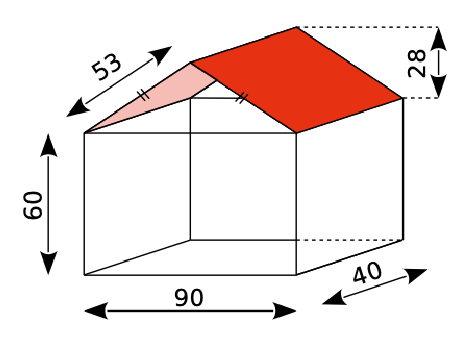
\includegraphics[width=50mm]{maison}
   \end{center}
   \vspace*{-5mm}
   \begin{enumerate}
      \item Calculer la surface de bois nécessaire pour réaliser le modèle de la maison.
      \item Sachant que le contre-plaqué choisi coûte \ueuro{28,90} le \umq{}, calculer le montant de sa dépense.
      \item Calculer, au \udmc{} près, le volume de la maison.
   \end{enumerate}
\end{exercice}

\begin{corrige}
   \ \\ [-5mm]
   \begin{enumerate}
      \item On a les pièces suivantes, les aires sont en \ucmq{} :
         \begin{itemize}
            \item fond : $90\times40 =3\,600$ ;
            \item face et arrière : $2\times(90\times60) =10\,800$ ;
            \item côtés : $2\times(40\times60) =4\,800$ ; 
            \item toit : $2\times(40\times53) =4\,240$ ; \smallskip
            \item pignons : $2\times\dfrac{90\times28}{2} =2\,520$. \smallskip
         \end{itemize}
         On additionne les mesures de toutes les pièces : \\
         $3\,600+10\,800+4\,800+4\,240+2\,520 =25\,960$. \\
         {\blue Il faut \umq{2,596} de bois pour la maison}.
      \item $2,596\times28,9 \approx75,02$. 
      {\blue Le prix est de \approx\ueuro{75}}.
      \item La maison a la forme d'un prisme de base : \\
      \ucmq{5400} + \ucmq{1260} = \ucmq{6660} et dont la hauteur vaut \ucm{40}. Son volume est donc de $\ucmq{6660}\times\ucm{40} =\ucmc{266400} =\udmc{266,4}$. \\
      {\blue Le volume de la maison est d'environ \udmc{266}}.
   \end{enumerate}
\end{corrige}

\end{colonne*exercice}


%%%%%%%%%%%%%%%%%%%%%%%%%%%%%%
%%%%%%%%%%%%%%%%%%%%%%%%%%%%%%
\Recreation

\begin{enigme}[Format A5 et cylindres]
   \partie[construction de cylindres]
   \ \\ [-10mm]
      \begin{enumerate}
         \item Découper une feuille au format A4 suivant sa médiane la plus courte afin d'obtenir deux feuilles au format A5.
            \begin{center}
               \begin{pspicture}(0,0)(3,2.3)
                  \psframe(0,0)(3,2.1)
                  \psline[linestyle=dashed](1.5,0)(1.5,2)
                  \rput(0.75,1){A5}
                  \rput(2.25,1){A5}
               \end{pspicture}
            \end{center}
         \begin{multicols}{2}
         \item Rouler la première feuille dans le sens de la \\
            longueur pour former un premier cylindre. \\
            {\psset{unit=0.7}
               \begin{pspicture}(0.5,-0.5)(11,3.75)
                  \psframe(0,0)(3,2.1)
                  \rput(1.5,1){A5}
                  \rput(4,1){$\Rightarrow$}
                  \psline(5.6,-0.37)(5.6,1.65)
                  \psline(5,0)(5,2)
                  \psline(7,0)(7,2)
                  \psellipticarc(6,2)(1,0.4){0}{-137}
                  \psellipticarc(6,0)(1,0.4){0}{137}
                  \psellipticarc(6,0)(1,0.4){180}{-137}
                  \rput(8,1){$\Rightarrow$}
                  \psline(10.5,0)(10.5,2)
                  \psline(9,0)(9,2)
                  \psellipse(9.75,2)(0.75,0.3)
                  \psellipticarc(9.75,0)(0.75,0.3){180}{0}
               \end{pspicture}}
         \item Rouler la deuxième feuille dans le sens de la \\
            largeur pour former un deuxième cylindre. \\
            {\psset{unit=0.71}
               \begin{pspicture}(0,-0.5)(8.5,3.75)
                  \psframe(0,0)(2.1,3)
                  \rput(1,1.5){A5}
                  \rput(3,1.5){$\Rightarrow$}
                  \psline(4.4,-0.3)(4.4,2.7)
                  \psline(4,0)(4,3)
                  \psline(5.5,0)(5.5,3)
                  \psellipticarc(4.75,3)(0.75,0.35){0}{-137}
                  \psellipticarc(4.75,0)(0.75,0.35){0}{137}
                  \psellipticarc(4.75,0)(0.75,0.35){180}{-137}
                  \rput(6.5,1.5){$\Rightarrow$}
                  \psline(8.5,0)(8.5,3)
                  \psline(7.5,0)(7.5,3)
                  \psellipse(8,3)(0.5,0.25)
                  \psellipticarc(8,0)(0.5,0.25){180}{0}
               \end{pspicture}}
         \end{multicols}
         \item À votre avis, ces cylindres ont-il le même volume ? Si non, quel est celui qui semble avoir le volume le plus grand ? \pointilles
      \end{enumerate}
      
   \partie[calcul du volume]
   \ \\ [-10mm]
   \begin{enumerate}
     \setcounter{enumi}{4}
        \item Rappeler les dimensions d'une feuille au format A4. En déduire les dimensions d'une feuille au format A5. \par \smallskip
           \pointilles \medskip
        \item Premier cylindre.
        \begin{enumerate}
           \item Donner la mesure de la hauteur du cylindre. \pointilles \\
           \item Que vaut le périmètre du disque de base du cylindre ? En déduire son rayon. \par \smallskip
           \pointilles \medskip
           \item Calculer alors  le volume du premier cylindre. \par \smallskip
           \pointilles \\
        \end{enumerate}
        \item Deuxième cylindre.
        \begin{enumerate}
           \item Donner la mesure de la hauteur du cylindre. \pointilles \\
           \item Que vaut le périmètre du disque de base du cylindre ? En déduire son rayon. \par \smallskip
           \pointilles \medskip
           \item Calculer alors  le volume du deuxième cylindre. \par \smallskip
           \pointilles \bigskip
        \end{enumerate}
        \item Conclusion : \pointilles \par \medskip
           \pointilles
     \end{enumerate}
\end{enigme}

\begin{corrige}
\begin{enumerate}
   \setcounter{enumi}{4}
      \item Format A4 : {\blue $\ell =\ucm{21}; L=\ucm{29,7}$}. \\
         Format A5 : {\blue $\ell =\ucm{29,7}\div2 = \ucm{14,85}; L=\ucm{21}$}.
      \item
      \begin{enumerate}
         \item La hauteur vaut {\blue $h_1 =\ucm{14,85}$}.
         \item Le périmètre du disque vaut {\blue $P_1 =\ucm{21}$}. \\
         Or, le périmètre d'un disque se calcule grâce à la formule $2\pi\times R$ où $R$ est le rayon du disque. \\
            Donc,  ${\blue R_1} =\ucm{21}\div(2\pi) {\blue \approx\ucm{3,34}}$.
         \item $\mathcal{V}_1 =\pi\times R_1^2\times h_1 \approx\pi\times(\ucm{3,34})^2\times\ucm{14,85}$ \\
            {\blue $\mathcal{V}_1 \approx\ucmc{520,44}$}.
      \end{enumerate}
      \setcounter{enumi}{6}
      \item
      \begin{enumerate}
         \item La hauteur vaut {\blue $h_2 =\ucm{21}$}.
         \item Le périmètre du disque vaut {\blue $P_2 =\ucm{14,85}$}. \\
            Donc,  ${\blue R_2} =\ucm{14,85}\div(2\pi) {\blue \approx\ucm{2,36}}$.
         \item $\mathcal{V}_2 =\pi\times R_2^2\times h_2 \approx\pi\times(\ucm{2,36})^2\times\ucm{21}$ \\
            {\blue $\mathcal{V}_2 \approx\ucmc{367,45}$}.
      \end{enumerate}
      \setcounter{enumi}{7}
      \item {\blue Le premier cylindre a le volume le plus grand}, malgré la feuille identique.
   \end{enumerate}
\end{corrige}
